\documentclass[11pt]{article}

\usepackage[margin=1.2in]{geometry}
%\usepackage{supertabular}
%\usepackage{setspace}
%\doublespacing
\usepackage{graphicx}
%\usepackage{hyperref}

\newcommand{\company}[1]{\verb|#1|}
\newcommand{\file}[1]{\texttt{#1}}
\newcommand{\program}[1]{\texttt{#1}}
\newcommand{\software}[1]{\verb|#1|}
\newcommand{\project}[1]{\texttt{#1}}
\newcommand{\comment}[1]{ [ \textit{#1} ] }

\newcommand{\DD}{\mathcal{D}}
\newcommand{\WW}{\mathcal{W}}
\newcommand{\TT}{\mathcal{T}}

\author{Ivan Savov}
\title{ {\LARGE Latent Dirichlet Allocation for \\ scientific topic extraction } }

\begin{document}
\maketitle

\abstract{
    We experiment with an automated topic extraction algorithm based on a generative graphical model.
    %learn a topic model from a large collection of scientific articles using 
    Latent Dirichlet Allocation assumes that individual words that appear in a document collection
    are drawn form a family of distibutions associated with a fixed number of topics. 
    We automatically learn these word-topic distributions from a collection of 20000 physics journal articles:
    % The data set is 
    the fulltext of the \texttt{arXiv.org/quant-ph} preprint archive between the years 1994 and 2007.
    We evaluate our results using the perplexity measure on the document collection.

    %We represent each document as an array of word counts from a fixed dictionary of size $W=?$,
    %which we determined by 
    %We display the discovered topics and incorporate them into a rudimentary recommendation system.
}

\ \\
\noindent {\bf keywords: } LDA, topic model, Gibbs sampling, clustering 
           % collapsed variational bayes, domain knowledge, 


\section{Introduction}

    There is a growing amount of unstructured data becoming freely available on the web and
    through various digitizaiton efforts.
    Due to the enormous scale of these data collections it is unrealistic to assume human
    supervision can play any significant role in their classification and curatorship.
    Clearly, automated largely-unsupervised machine learning techniques will be required
    in order to deal with the information oveload.

    The subjects of classification, retreival and browsing have been central topics of research
    in the data mining community for the past decade, but there is still more work to be done.
    Recently, there has been a surge of interest in the machine learning community about
    ``topic models'' which attempt to automatically extract the subject matter from
    document collections \cite{Blei2003,Blei2009}.
    These techniques are scalable to very large document collections and produce very informative
    results despite using the same old data mining paradigm of representing each document as bag of words.

    For this project we will focus our attention on the \emph{latent Dirichlet allocation} (LDA) model
    which is described in the seminal paper by Blei, Ng and Jordan \cite{Blei2003}. 
    %This is the original proposal that kick-started the recent interest in topic models.
    %The original paper uses variational methods to learn the model parameters which can be s, but 
    We will use a Gibbs sampling approach to learn the LDA parameters which is very computationally
    efficient \cite{griffiths2004finding}. 
    Computaitonal efficiency will be important since our data set contains rougly 20k documents and 
    which are represented as word counts of over a dictionry of 10k words.
    
    This report is structured as follows.
    In the next section we will provide some theoretical background on the LDA model.
    Afterwards, we will discuss the inference procedure we used to learn the model parameters.
    Section \ref{section:data-set} is describes our data set and the preprocessing we performed.
    We descirbe the results of two experiments in seciton \ref{section:results} and follow up
    with a some discussion and a conclusion.



\section{The model}

    Terms to discuss MAP, PLSA, VB, CVB0 etc...
    LDA 
    \begin{figure}[htb]
    \begin{center}
    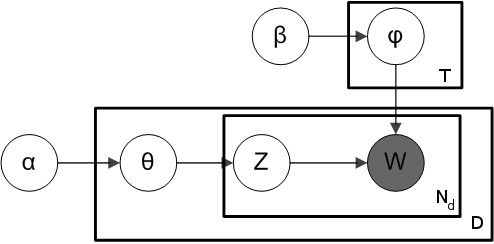
\includegraphics[width=3in]{lda-diagram.png}  %[height=1in,width=1in,angle=-90]{foo}
    \caption{ The graphical model behind LDA. $\theta$ is the distribution  of topics for a document,
              $\beta$ is the distribution of words for a given topic.}
    \end{center}
    \end{figure}


\section{The inference algorithm}

    First we being by definiting some quantities
    
    We have the document set $\DD = \{ d_1, d_2, \ldots, d_D \}$, where each document consists of 
    a word count vector for the words taken from a fixed vocabulary $\WW$ of size $W$.
    
    Our aim is to produce a set of topics $\TT$ where each topic is a probability distribution over words $\WW$.
    
    
    \begin{description}
	\item[$\gamma_{wjk}$:]	$=Pr( z=k | x=w,d=j)$, the probability that word $w$ in document $j$ 
						is assigned to the topic k.
	\item[$N_{wj}$:]	\# of times $w$ appears in doc $j$. 
	\item[$N_{wk}$:]  $=\displaystyle\sum_{j\in \DD} N_{wj}\gamma_{wjk} = $ \# of times $w$ appears in topic $k$.
	\item[$N_{kj}$:]  $=\displaystyle\sum_{w\in \WW} N_{wj}\gamma_{wjk} = $ \# of times topic $k$ appears in doc $j$.
	\item[$N_{k}$:]  $=\displaystyle\sum_{w\in \WW} N_{wk}=  \displaystyle\sum_{w\in \WW}\sum_{j\in \DD} N_{wj}\gamma_{wjk} $ \# words assigned to  topic $k$.
	\item[$N_{j}$: ]  $=\displaystyle\sum_{k \in \TT} N_{kj} =  \displaystyle\sum_{k \in \TT}\sum_{w\in \WW}N_{wj}\gamma_{wjk} $ \# words in doc $j$.
    \end{description}


    To achieve this we will have to learn...


\section{The data set} \label{section:data-set}

	The good people who run the arXiv.org were kind enough to send me the entire collection of papers
	in the \texttt{quant-ph} repository! 
    The arXiv is a prominent publication in the physicsl sciences and contains pre-print versions
    of most of the important research in several areas.
    Of particular interest is the field of quantum information science which is very well
    represented.
	
    The raw data that was received consists of two directories. 
    The first directory, \file{pdf/} of size 7.1GB condains 31739 pdf documents.
    The second directory \file{tex/}  contains the \LaTeX \ source code of some of the papers 
    (its size is 2.1G and it contains 21061 files). 
    Since the source code of only about $2/3$ of the papers was available, we decided to use 
    the pdf version of the document collection.

%	\begin{verbatim}
%	ivan@flicker:/scratch/arxiv$ du -sh *
%	7.1G    pdf
%	2.1G    tex
%	ivan@flicker:/scratch/arxiv$ find pdf/ -type f | wc
%	31739   31739  730019
%	ivan@flicker:/scratch/arxiv$ find tex/ -type f | wc
%	21061   21061  470945
%	\end{verbatim}
	
%	The \texttt{pdf/} directory contains the pdf versions of the papers and for some of these papers.
%	For about $2/3$ of these we also have the latex source code in the \texttt{tex/} directory.
	
	Some more information about the raw dataset.
	\begin{itemize}
		\item Total number of pdf files: 31739
        \item Total number of papers: 20166 (multiple versions v1,v2)
        \item Number of files with unreadable/foreign fonts: 6
		\item Earliest date: 22 Dec 1994  (pdf/9412/9412002v1.pdf)
		\item Most recent:  30 Mar 2007 (pdf/0703/0703278v1.pdf)
	\end{itemize}
	
	
	
	\subsection{Textual pre-processing}

        Since the intended feature vectors are word counts, we used the command-line utility
        \texttt{pdftotext} (part of \program{xpdf}) to convert the pdf documents to text files.
        The python script \file{preprocessing/pdftotext.py} accomplishes this and stores the
        output in the folder \file{data/text} while at the same time creating an inventory of
        all the available documents.
        At this stage, some documents were found to be unreadable or used foreign language fonts
        which were not recognized by xpdf. There were very few such documents so it was possible
        to manually remove them from the inventory.

        At this point we had 31732 documents in our ``inventory'', but some of these documents
        were different version of the same underlying paper (ex: \file{9412002v1.pdf},
        \file{9412002v2.pdf}, etc.).
        We therefore ran \program{dupremover.py} which kept only the latest version.
        After this step, the total number of papers in our data set decreased to 20166.

        Before we can perform any word counts, however, we had to deal with a typographical issue.
        Ligatures are linkages between the letters f, l and i in high quality fonts.
        Since \LaTeX \ uses the computer modern fonts which have ligatures, the document collection
        was full of them. For example, when I write the word ``affluent'' it will not be treanlsated
        into the sequence of characters a,f,f,l,u,e,n,t but instead turn into a,ffl,u,e,n,t where 
        ffl is a single unicode character. Can you see the difference between ffl and f{}f{}l?
        In order to deal with this issue, I did a preliminary pass using \program{makewordstream.py}
        expanding all ligatures to their consitituent letters. 
        While I was at it, I also converted all words to lowercase ASCII.
		  

    \subsection{Dictionary selection}

        The next step was to select a subset of all the words that occur in the document collection
        for which we will perform word count.
		I first pass was made on the documents to remove a standard list of stopwords (see
        \file{stopwords.py}). 
		Given how large the dataset is we did not feel it was necessay to use word stemming;
        this way we can capture as much of the granularity of the data as possible.

        The total number of unique words of 3 character or more at this step was 67075, and
        contained lots of non-words like ``ijk'', which probably refer to matrix indices.
        While 60k words is not an unreasonable dictionary size, it was deemed too large for
        our purposes and an effort was made to cut down on the dictionary size.
        The script \program{makevocab.py} goes through the word stream and counts total
        number of occurences for each word. It then rejects all words that occur less than
        45 times in the corpus. 
        We also impose a minimum occurence threshold of 10000, 6000 and 2000 for three, four and
        five letter words respectively.

        The final pre-processing step selects the top 10011 words by overall frequency 
        and stores it in the file \file{vocab.txt}.
        This figure was inspired by the paper \cite{Blei2009}, where they use a vocabulary of this
        size on a document collection roughly similar to our own.


    \subsection{Sparse matrix format}

        The input data that the \program{topicmodel} program expects is in a standard sparse 
        matrix format which is generated by the script \program{Makedocword.pl}.
        The resultting file \file{docword.txt} contains one row for each unique word
        in each document. For example, consider the following exerpt:
        \begin{verbatim}
        #docword.txt
        ...
        34 376 6
        34 6767 5
        ...
        \end{verbatim}
        These two lines indicate that the document with id=34 contains 6 occurences of word 376
        and 5 occerences of word 6767.
        This is the standard bag-of-words paradigm for each document.
        %    folder + symlinks\\


    The following list summarizes the important details of the finalized data set 
    at the stage when it is read to be fed to the Gibbs sampling inference algorithm.
	\begin{itemize}
        \item Size of vocabulary: $W=10011$  
        \item Total number of documents: $D=20166$ 
        \item Total number of words in corpus: $N=41202148$
          %\item Total number of unique words: $N=11220266$
	\end{itemize}



\section{Results} \label{section:results}
	

    The natural application of topic models is the automated extraction of topics from
    the data set. 
    Given that we have learned the 


    Another, more scientific method for evaluating the performance of a topic model 
    is to calulate the perplexity.
    \begin{equation}
        pplex\!\left(\DD\right) = \exp\left( - \frac{1}{N} \sum_1^N \log P(w_n|d_n) \right),
    \end{equation}



    See how to classify new documents.
    Calculate perplexity and KL distance for different runs with same parameters

    \subsection{Informal evaluation of extracted topics}

        list them all....


    \subsection{Number of topics}



    \subsection{Gibbs sampling chain length}

    Compare for different NITER and Ntopics
        The 


	I will read the original 2003 paper by Blei, Ng and Jordan \cite{Blei2003} and also perform a general literature
	review on topic models.
	In particular, I want to verify the results of the ICML09 paper \cite{Teh2009} which state that all the different 
	models of training
	LDA are equivalent and only differ by the setting of the hyper-parameters.
	
	I will try to implement the Collapsed Variational Bayes technique of \cite{Teh2007}.
	
	The results I would like to obtain is some meaningful cluster structure over the scientific topics.
	
    run it and time it \\ 
    check memory usage as it runs \\
	
	
\section{Discussion and future work}

	\subsection{Regular expressions}
	
		This could be a study of what you can do with different features.
		We can have as higher level features counts from regular expression matches.
		These features can themselves be refined over generations or by cross validation.
		
		Come to think of it you can do all kinds of things with this.
		Regular expressions of the form "quantum (mechanics|physics)" for compound words 
		that are synonymous. 
		
		Algorithm: Self-refining regular expression features
		\begin{enumerate}
			\item	Start with word counts for a fixed list of words of size $|W|$ and do regular LDA.
			\item	For each of the latent topics build all "two word" combinations.
			\item	Rerun LDA on the expanded feature space of size $|W|^2 + |W|$.
			\item	Find the important second order occurrences and discard all other features.
			\item	Try to compress multiple variations using regular expression language. \\
					Example: "a b", "a c", "a d"  can be converted into regex "a (b|c|d)"
			\item	Go to step 3 but now number of features is $|W|+$ n\_of\_good\_reg\_exes
		\end{enumerate}

		I am not sure if this will generate all possible word occurences but I think reg-exes are
		pretty rich as feature set and their computation is all paralelizable so it doesn't matter if 
		it is very expensive.
		
		
		Can we let some genetic algorithm work on this instead?



    \subsection{Two data set correlations}

        You browse wikipedia about quantum informaiton topics and it suggests
        papers that are most similar to the subject --- not so useful.

        Maybe the opposite is better, as you browse the arXiv you get suggested
        links to articles on wikipedia that cover similar topics.




	
	\subsection{This paper covers}
	
		User interface idea: papers laid out on a table in such a way that the papers that
		cite each other overlap. All papers in the same "epoch" are visible at the same time
		and placement and paper size indicates relative importance.
		
		(One way to think about this is where are the words of this each topic passed on from one generation
		to the next)
		 
		
	\subsection{CUDA }
			
    \subsection{Citaiton graph}
        We can use a simple reg-ex to match things like \\
        \verb| quant-?ph\d{7} | and extract all citations to other
        papers on the archive.
        It won't be very complete, but you can still extract a sense 
        of importance from it !
        page rank ;)

    \section{Metadata}
        We should have the titles for each of these articles I think
        we need a little urllib2 script to get each of
        \verb|http://arxiv.org/list/quant-ph/0003?show=1000|
        where 0003 corresponds to my folder 0003 


\section{Conclusion}

    We have demonstrated that     


\bibliographystyle{alpha}
\bibliography{arXivLDA}


\end{document}
